\documentclass[12pt,a4paper]{article}

% \newcommand*{\TypeChinese}{} % Chinese support
\newcommand*{\AdvancedDocument}{} % include code and math
\newcommand*{\WithHeader}{}

% basic packages
\usepackage[margin=2cm]{geometry}
\usepackage{graphicx,subfigure,indentfirst,hyperref,colortbl,caption,cite,color,xcolor,tikz}
\hypersetup{colorlinks=true,urlcolor=blue,linkcolor=blue}

\ifdefined\AdvancedDocument
	% minted is better than listing.
	\usepackage{minted}
	% it requires minted of a newer version.
	\setminted{linenos=true, frame=lines, framesep=2mm}	
	\usepackage{amsmath,amssymb,bm}
\fi

\ifdefined\TypeChinese
	\usepackage{xeCJK,fontspec}
	\XeTeXlinebreaklocale "zh"
	\XeTeXlinebreakskip = 0pt plus 1pt
	\setmainfont{KaiGen Gothic TW}
	\setCJKmainfont{KaiGen Gothic TW}
	\setmonofont{Droid Sans Mono}
	\renewcommand{\baselinestretch}{1.3}
\fi

\ifdefined\WithHeader
	\usepackage{fancyhdr}
	\fancypagestyle{plain}{
		\fancyhf{}
		\chead{GPU Programming 2018 Spring \textbar ~CSIE Department, National Taiwan University}
		\cfoot{\thepage}
		\rfoot{GPGPU Assignment \#3}
	}
	\pagestyle{plain}
	\renewcommand{\headrulewidth}{1pt}
	\renewcommand{\footrulewidth}{2pt}
\fi

\newcommand{\figref}[1]{Figure \ref{fig:#1}}
\newcommand{\tabref}[1]{Table \ref{tab:#1}}
\newcommand{\equref}[1]{Equation \ref{equ:#1}}
\newcommand{\lstref}[1]{Listing \ref{lst:#1}}
\graphicspath{{jpg/}}

\begin{document}
\title{GPGPU Assignment \#3}
\author{Author: Yu-Sheng Lin \and Instructor: Wei-Chao Chen}
\maketitle

\section{Goals}

Implement Poisson Editing for image cloning on the GPUs.  Go fancy and implement faster algorithms to gain the bonus points.

\section{Description}

\subsection{Image Cloning}

\figref{img_clone} shows input examples for image cloning algorithms, where
(a) is the background, (b) is the target image, and (c) is a boolean mask.
You may perform naive image cloning such as \figref{img_clone_example} by 
copying and pasting the image from the target image
to the background image according to the binary mask.
This algorithm is provided in the sample codes.

Obviously there are rooms for improvement from this naive algorithm.
In this assignment, we ask you to implement Poisson Editing, 
a computationally intensive but effective algorithm that is designed to seamlessly blend the background
and target images by means of differential domain operations.
The algorithm is described in more details later in this document, and 
we encourage you to read the original paper \textit{Poisson Image Editing} from SIGGRAPH 2003 by P. Perez et al.

\subsection{Function Signature}

The function signature for this assignment is \lstref{sig}.
\verb+background+ and \verb+output+ are
interlaced RGB images of size $W_b\times H_b$ and
range from $0$ to $255$.
\verb+target+ is the same except that its size is $W_t\times H_t$.
\verb+mask+ is the mask that contains only one color channel and
we use \verb+0.0f/255.0f+ to represent false/true.

\begin{listing}[ht]
\begin{minted}{cpp}
void PoissonImageCloning(
    const float *background,
    const float *target,
    const float *mask,
    float *output,
    const int wb, const int hb, const int wt, const int ht,
    const int oy, const int ox
);
\end{minted}
\caption{Function signature}\label{lst:sig}
\end{listing}

We will also assign the offset $O_y, O_x$,
which means the offset of the target image
in the background image (from the top-left corner),
and we will test your program using these two commands.

\begin{listing}[ht]
\begin{minted}{bash}
./a.out img_background.ppm img_target.ppm img_mask.pgm 130 600 output.ppm
./a.out img_background.ppm img_target.ppm img_mask.pgm 130 900 output.ppm
\end{minted}
\caption{Execute your code}\label{lst:exe}
\end{listing}

We use the very popular PGM/PPM image format,
which can be edited by many image processing softwares.
You can generate new test cases if you wish.

\subsection{Poisson Editing}

\begin{figure}
\centering
\subfigure[The background image $W_b\times H_b$.]{\includegraphics[width=0.6\textwidth]{img_background.jpg}}\\
\subfigure[The target image which will be pasted to the background, $W_t\times H_t$.]{\includegraphics[width=0.35\textwidth]{img_target.jpg}}
\subfigure[The mask $W_t\times H_t$.]{\includegraphics[width=0.35\textwidth]{img_mask.jpg}}
\caption{The input images of this assignment.}\label{fig:img_clone}
\end{figure}

\begin{figure}
\centering
\includegraphics[width=0.6\textwidth]{output.jpg}
\caption{A very naive and ineffective image cloning output.}\label{fig:img_clone_example}
\end{figure}

\begin{figure}
\centering
\subfigure[The values to be solved.]{
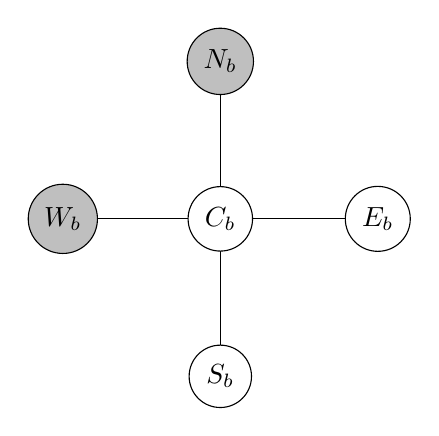
\begin{tikzpicture}[scale=1]
\coordinate (C) at (2,2);
\coordinate (N) at (2,4);
\coordinate (W) at (0,2);
\coordinate (S) at (2,0);
\coordinate (E) at (4,2);
\draw (C) -- (W);
\draw (C) -- (N);
\draw (C) -- (W);
\draw (C) -- (S);
\draw (C) -- (E);
\node[circle,draw,fill=white] at (C){$C_b$};
\node[circle,draw,fill=lightgray] at (N){$N_b$};
\node[circle,draw,fill=lightgray] at (W){$W_b$};
\node[circle,draw,fill=white] at (S){$S_b$};
\node[circle,draw,fill=white] at (E){$E_b$};
\end{tikzpicture}
}
\hspace{1.5cm}
\subfigure[The corresponding target image.]{
\begin{tikzpicture}[scale=1]
\coordinate (C) at (2,2);
\coordinate (N) at (2,4);
\coordinate (W) at (0,2);
\coordinate (S) at (2,0);
\coordinate (E) at (4,2);
\draw (C) -- (W);
\draw (C) -- (N);
\draw (C) -- (W);
\draw (C) -- (S);
\draw (C) -- (E);
\node[circle,draw,fill=white] at (C){$C_t$};
\node[circle,draw,fill=white] at (N){$N_t$};
\node[circle,draw,fill=white] at (W){$W_t$};
\node[circle,draw,fill=white] at (S){$S_t$};
\node[circle,draw,fill=white] at (E){$E_t$};
\end{tikzpicture}
}
\caption{The gray nodes are the boundary (the black pixels in the mask).}\label{fig:linear_sys}
\end{figure}

If you wish to bypass the mathematical details in the original paper, 
you may proceed by implementing this 4-neighbor linear system in
\equref{linear_sys} (also refer to \figref{linear_sys}).

\begin{equation}
4C_b - (S_b+E_b) = 4C_t-(N_t+W_t+S_t+E_t) + (N_b+W_b).
\label{equ:linear_sys}
\end{equation}

With the \textbf{Jacobi Iteration}, the iteration step is in \equref{jacob},
where $C_b'$ is the value of the next step and $S_b, E_b$ is the value of current step.
You may also notice that $C_b'$ is independent of $C_b$
but only depends on it's neighbors.

\begin{equation}
C_b' =
\frac{1}{4} \left[
	\underbrace{4C_t-(N_t+W_t+S_t+E_t) + (N_b+W_b)}_\text{Fixed during iterations}
	+ \underbrace{(S_b+E_b)}_\text{Current value}
\right]
\label{equ:jacob}
\end{equation}

It is your job to generalize and figure out the equation for (1) when the locations of gray points change, and (2) when the point has less than four neighbors.

\subsection{Acceleration}

This part is counted as bonus.
To qualify for the bonus, you would also need to write a short report about your speed up and implementation.
You may, for example, compare convergence against the number of iterations or execution time.
We describe a few possible speed-up mechanisms, and our conjectures about how much you may gain from implementing these suggestions.

First, you may observe that
the time for a value to propagate from the left to the right of the image
is proportional to the width of the image.
Therefore it may require the square of image sizes to actually converge to a proper solution.
A naive implementation would require thousands of iterations to converge,
which is very impractical.
\figref{convergence} shows results with TA's baseline implementation.
As you can see, it takes 20000 iterations to converge.

A cheaper solution is to use a hierarchical method.
Start by solving the problem at a lower resolution, upsample, and then solve it at a higher resolution.
You could do this at $1/8$x, $1/4$x, $1/2$x and $1$x scales with the nearest-neighbor upsampling algorithm, for example.
Note that the number of iterations after each scale promotion would be less than solving the complete problem, because your lower-resolution solutions would look reasonably similar to the higher resolution ones already.

\begin{figure}
\centering
\subfigure[2 iterations]{\includegraphics[width=0.45\textwidth]{2.jpg}}
\subfigure[20 iterations]{\includegraphics[width=0.45\textwidth]{20.jpg}}\\
\subfigure[200 iterations]{\includegraphics[width=0.45\textwidth]{200.jpg}}
\subfigure[2000 iterations]{\includegraphics[width=0.45\textwidth]{2000.jpg}}\\
\subfigure[6000 iterations]{\includegraphics[width=0.45\textwidth]{6000.jpg}}
\subfigure[20000 iterations]{\includegraphics[width=0.45\textwidth]{20000.jpg}}
\caption{The convergence with Jacobi Iteration.}\label{fig:convergence}
\end{figure}

You may also try the \textbf{successive over-relaxation method (SOR)},
which changes the iteration steps to \equref{sor},

\begin{equation}
C_{b,SOR}' = \omega C_b + (1-\omega) C_{b,SOR}.
\label{equ:sor}
\end{equation}

SOR is just a interpolation/extrapolation between
current values and the values of the next iteration.
Sadly, since the linear system is not \textbf{diagonally dominant},
the SOR Jacobi iteration diverges.
(In fact, even na\"ive Jacobi iteration is not guaranteed to converge.)
However, some students of 2017 accidentally found that the following
alternative formula works perfectly in this assignment.

\begin{equation}
C_{b,SOR}'' = \omega C_b' + (1-\omega) C_{b,SOR}.
\label{equ:sor_modify}
\end{equation}

The new formula extrapolates against the $C_b$ two steps before,
instead of one, and this can still be implemented without an third buffer.
We have confirmed that $\omega = 1.9$ works fine.

\section{Grading}
\begin{enumerate}
\item 100 points, when you finish the baseline implementation (Jacobi, no acceleration).
\item Up to 20 bonus points for SOR Jacobi.
\item Up to 40 bonus points for hierarchical Jacobi.
\item Up to 50 bonus points if you can tell why Equation \ref{equ:sor_modify} works magically.
\item Up to 50 extra bonus points for any other speed-up implementation.
\end{enumerate}

\section{Submission}
\begin{itemize}
	\item The submission deadline is 2018/05/31 23:59 (Fri.).
\item Please submit the result in loseless PNG format \verb+lab3/results/***.png+.
\item Submit your source code \verb+lab3/lab3.cu+. Again, you should only modify this file in the homework.
\item We will test your code with the command listed in \lstref{exe}.
\item If you implement hierarchical, SOR, or any other speed-up algorithm, you need to submit a report \verb+lab3/report.pdf+ to be considered for the bonus.
\end{itemize}

\section{Hint}
\lstref{hint} contains part of TA's baseline code. Feel free to use it.

\pagebreak

\begin{listing}
\begin{minted}{cpp}
void PoissonImageCloning(
   const float *background,
   const float *target,
   const float *mask,
   float *output,
   const int wb, const int hb, const int wt, const int ht,
   const int oy, const int ox
) {
   // set up
   float *fixed, *buf1, *buf2;
   cudaMalloc(&fixed, 3*wt*ht*sizeof(float));
   cudaMalloc(&buf1, 3*wt*ht*sizeof(float));
   cudaMalloc(&buf2, 3*wt*ht*sizeof(float));

   // initialize the iteration
   dim3 gdim(CeilDiv(wt,32), CeilDiv(ht,16)), bdim(32,16);
   CalculateFixed<<<gdim, bdim>>>(
      background, target, mask, fixed,
      wb, hb, wt, ht, oy, ox
   );
   cudaMemcpy(buf1, target, sizeof(float)*3*wt*ht, cudaMemcpyDeviceToDevice);

   // iterate
   for (int i = 0; i < 10000; ++i) {
      PoissonImageCloningIteration<<<gdim, bdim>>>(
         fixed, mask, buf1, buf2, wt, ht
      );
      PoissonImageCloningIteration<<<gdim, bdim>>>(
         fixed, mask, buf2, buf1, wt, ht
      );
   }

   // copy the image back
   cudaMemcpy(output, background, wb*hb*sizeof(float)*3, cudaMemcpyDeviceToDevice);
   SimpleClone<<<gdim, bdim>>>(
      background, buf1, mask, output,
      wb, hb, wt, ht, oy, ox
   );

   // clean up
   cudaFree(fixed);
   cudaFree(buf1);
   cudaFree(buf2);
}
\end{minted}
\caption{Hint}\label{lst:hint}
\end{listing}

\end{document}
